\chapter{Underground Excavation}
\label{ch:fscf-excav}

The main excavated spaces necessary to support the LBNF experiment are a combination of excavations required for the experiment and those required for constructability. Experimental spaces on the 4850L include the detector chambers, drifts for access and utility routing, and the Central Utility Cavern. Spaces identified as likely necessary for the excavation subcontractor include mucking drifts connected to the Ross Shaft to enable waste rock handling and equipment assembly shops to provide space to assemble and maintain excavation equipment underground. In addition, a spray chamber is provided for heat rejection from the chilled water system. All spaces are identified on the 100\% Preliminary Design excavation drawings produced by Arup\cite{arup:fscf100pdr}. The spaces are shown below in Figure~\ref{fig:spaces-4850}.

\begin{cdrfigure}[Spaces required for LBNF at 4850L]{spaces-4850}{Spaces required for LBNF at 4850L (SURF)}
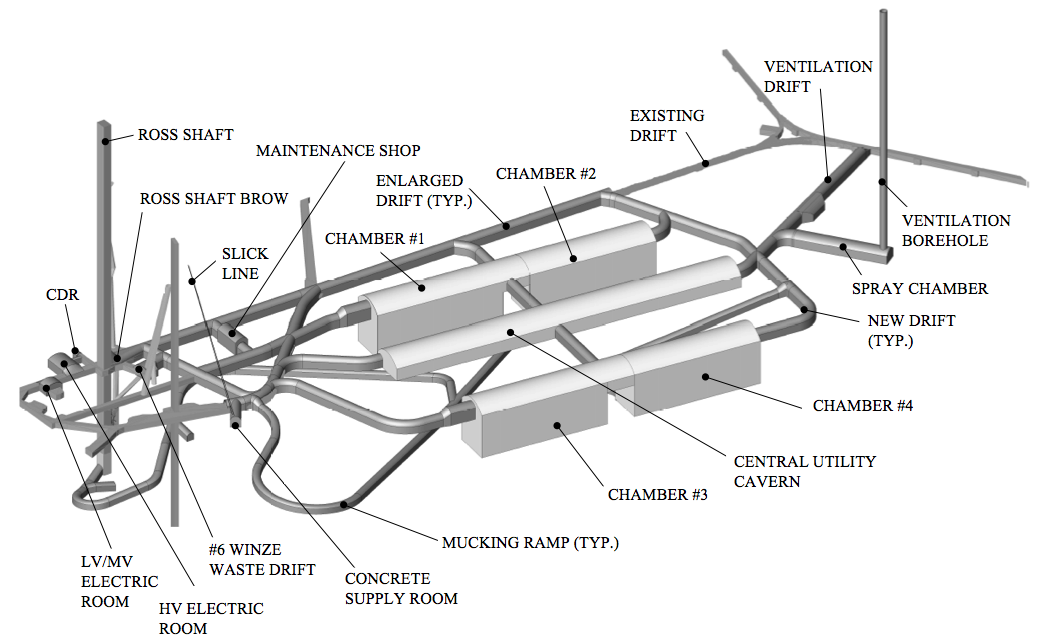
\includegraphics[width=\textwidth, angle=90]{spaces-4850}
\end{cdrfigure}

%%%%%%%%%%%%%%%%%%%%%%%%%%%%%%%%%%%%%%%%%%%%%%%%%%%%%%%%%%%%%%%%%%%
\section{LBNF Cavities}
\label{sec:fscf-excav-cav}

%%%%%%%%%%%%%%%%%%%%%%%%%%%%%%%%%%
\subsection{Detector Cavities}
\label{sec:fscf-excav-det}

The required experimental spaces were defined through interaction with the DUNE design team and are documented in LBNF Requirements Document [14]. The size and depth of the LBNF cavities were prescribed to suit the scientific needs of the experiment. The overall main cavern sizes are shown graphically in Figure~\ref{fig:dim-cavern-excav}. The DUNE experiment will be housed in four detector chambers within two main caverns at the 4850L. Siting deep underground is required to shield from cosmic rays, as detailed in Report on the Depth Requirements for a Massive Detector at Homestake [15]. The 4850L is deeper than what is absolutely required, but is used because of existing access at this level. 

\begin{cdrfigure}[Dimensions of the main LBNF cavern excavations]{dim-cavern-excav}{Dimensions of the main LBNF cavern excavations (final dimensions will be slightly smaller). (SURF) }
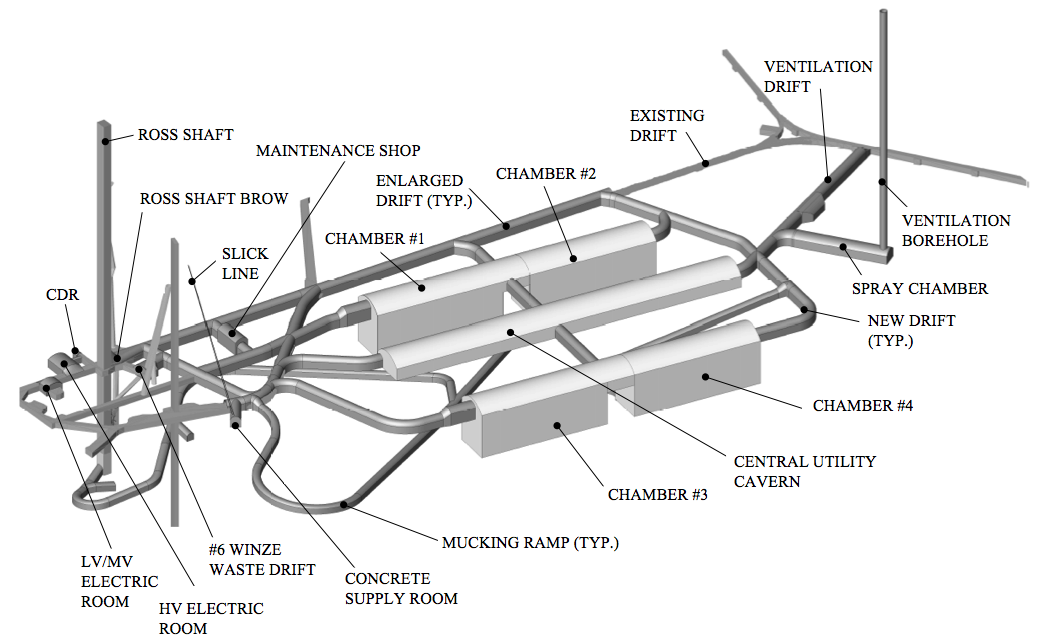
\includegraphics[width=0.9\textwidth]{dim-cavern-excav} 
\end{cdrfigure}

The limits on size for the detector are determined by rock strength and the limits on the ability to produce large dimension anode and cathode plane arrays. Space occupied by the free-standing steel structure, vessel insulating liner, and an intentional exclusion zone reduce the fiducial volume of the detector below the volume of the excavation. Current assessment of rock quality indicates that a cavity of this size is reasonable with the rock quality assumed for this formation.

Preliminary modeling of the proposed excavations included 2D and 3D numerical modeling. The intact rock strength and joint strength had the greatest impact according to the 2D modeling, and 3D modeling confirmed that the complex geometry is possible. 

The far detector cavity and drifts will be supported using galvanized rock bolts/cables, wire mesh, and shotcrete for a life of 30 years. The floor of the cavity has been evaluated and does not require support. 
A groundwater drainage system will be placed behind the shotcrete in the arch and walls of the far detector cavity rock excavation. This drain system will collect groundwater (native) seepage and eliminate the potential for hydrostatic pressure build-up behind the shotcrete. Channels will be placed in the concrete invert to drain groundwater to the sump system. 

%%%%%%%%%%%%%%%%%%%%%%%%%%%%%%%%%%
\subsection{Structure and Cranes}
\label{sec:fscf-excav-cranes}

The LBNF caverns require monorail cranes to facilitate the construction of the detector components. Rock bolts will be coordinated with the excavation contractor to provide anchorage to support these monorails.

%%%%%%%%%%%%%%%%%%%%%%%%%%%%%%%%%%%%%%%%%%%%%%%%%%%%%%%%%%%%%%%%%%%
\section{LBNF Central Utility Cavern}
\label{sec:fscf-excav-util-cav}

LBNF requires spaces for cryogenics equipment outside of the detector caverns. These requirements have been combined with that for the conventional facilities utilities in an independent Central Utility Cavern. This area will house the experiment's cryogen system, electrical equipment to supply power for facility and experiment needs, sump pump access and controls, fire sprinkler room, air handling units (AHUs), chilled water system, and ducting. The centralized location minimizes overall utility distribution costs. Isolating the utilities from the experiment simplifies electrical ground isolation to avoid interference with sensitive detector electronics, and also provides the opportunity to optimize ventilation to control heat emanating from the equipment in the Central Utility Caverns.

%%%%%%%%%%%%%%%%%%%%%%%%%%%%%%%%%%%%%%%%%%%%%%%%%%%%%%%%%%%%%%%%%%%
\section{Access/Egress Drifts}
\label{sec:fscf-excav-access-drifts}

In order to accommodate deliveries, the drift connections from the Ross Shaft to new excavations required for LBNF will be optimized to accommodate the maximum load size possible through the shaft plus the utilities required to service the facility. At the writing of this document, an assumed size of 5m wide by 6m tall is used for all access and egress drifts. All new excavations, or drifts enlarged for LBNF will be provided with a shotcrete wall (rib) and ceiling (back) and a concrete floor (sill).

%%%%%%%%%%%%%%%%%%%%%%%%%%%%%%%%%%%%%%%%%%%%%%%%%%%%%%%%%%%%%%%%%%%
\section{Excavation Sequencing}
\label{sec:fscf-excav-exc-seq}

A key goal of both LBNF and DUNE is to complete construction of one 10 kt detector as soon as possible. To facilitate this, the excavation will be sequenced to allow DUNE to begin installation of a cryostat in the first detector chamber while excavation continues. A temporary wall will be built in the detector installation laydown space between detector chambers to isolate one area from another. This wall must be of sturdy construction to withstand air shock waves associated with drill and blast type construction. Further evaluation of vibration limits and controls must be considered as the design advances to avoid damaging the cryostat during assembly.

In addition to controlling the impacts from blasting, logistical coordination is a key concern with a sequenced excavation allowing cryostat construction concurrent with excavation. Many experiment components will be delivered through the Ross shaft, competing with excavation and other construction. A logistics study\cite{lbnf-logistics} has been performed to evaluate whether this can be done without impact on either civil or experiment construction.  This study confirmed that with good coordination, led by the construction manager, this single shaft can support all anticipated material and personnel deliveries.  The Yates shaft can provide some relief during high intensity work periods as well, but this was not considered in the study to evaluate the most conservative approach.

Most excavated material will travel through a mucking ramp starting at the base of each detector pit and ending at the waste dump near the Ross Shaft. This route is completely independent of all other traffic and includes a separate ventilation stream to keep diesel exhaust from other occupied spaces. During times when excavation is establishing the upper sections of the caverns and developing a means of dumping excavated material to this lower elevation, material will need to be transported at the 4850L. To alleviate any potential interferences, the first phase of construction will establish a connection from the 4850L to the mucking ramp, as well as ventilation paths to avoid contaminating the air in spaces that have been turned over for cryostat construction. 

Delivery of cryostat components to the individual pits can be accomplished in one of two ways. All materials are delivered through the shafts to the 4850L, which is ~18m above the base of the pits. During construction of the first cryostat, while excavation continues in the other areas, all materials will be delivered to the detector installation laydown area between the first and second detector chambers and/or to the west end of the first detector chamber. An overhead crane will be used to lower this material into the pits. This crane is required for installation of detector component within the cryostat, so is not additional equipment. All excavation will be completed before any construction is required in the third and fourth detector pits, providing the opportunity to use the excavation mucking ramp for delivery of cryostat components. This ramp has been designed at an 8\% grade to from the west side to allow for this possibility. 

%%%%%%%%%%%%%%%%%%%%%%%%%%%%%%%%%%%%%%%%%%%%%%%%%%%%%%%%%%%%%%%%%%%
\section{Interfaces between DUNE, Cryogenics and Excavation}
\label{sec:fscf-excav-interfaces}

There are several points at which the experiment and the facility interface closely. These are managed through discussions between DUNE design team, the Cryogenics Infrastructure design team, and the Conventional Facilities design team and design consultants.
\begin{itemize}
\item The LBNF cryostat is a freestanding structure requiring infrequent access for inspection around the vessel. Low tolerance control in excavation will impact the cost of providing access to inspect this vessel.
\item The utility spaces to house the cryogen system are directly influenced by the size of the cryogen system equipment.
\item The size and construction sequencing of the detector chambers are critical to the experimental strategy.
\end{itemize}




